\subsection{« between »}
\begin{tcolorbox}[arc=5pt, colback=white!0, colframe=orange!50!black]
\infbox{
Insertion de \textbf{« between »}
}
\begin{center}
\tbox{
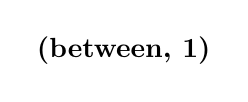
\begin{tikzpicture}
[
    level 1/.style={sibling distance=75mm},
    level 2/.style={sibling distance=35mm},
]
\node {\bfseries (between, 1)} 
;
\end{tikzpicture}
}
\end{center}

\end{tcolorbox}\subsection{« the »}
\begin{tcolorbox}[arc=5pt, colback=white!0, colframe=orange!50!black]
\infbox{
Insertion de \textbf{« the »}
}
\begin{center}
\tbox{
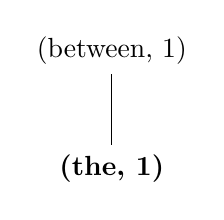
\begin{tikzpicture}
[
    level 1/.style={sibling distance=75mm},
    level 2/.style={sibling distance=35mm},
]
\node { (between, 1)} 
    child {node{\bfseries (the, 1)} 
};
\end{tikzpicture}
}
\end{center}

\end{tcolorbox}\subsection{« and »}
\begin{tcolorbox}[arc=5pt, colback=white!0, colframe=orange!50!black]
\infbox{
Insertion de \textbf{« and »}
}
\begin{center}
\tbox{
\begin{tikzpicture}
[
    level 1/.style={sibling distance=75mm},
    level 2/.style={sibling distance=35mm},
]
\node { (between, 1)} 
    child {node{\bfseries (and, 1)} 
}    child {node{ (the, 1)} 
};
\end{tikzpicture}
}
\end{center}

\end{tcolorbox}\subsection{« centuries »}
\begin{tcolorbox}[arc=5pt, colback=white!0, colframe=orange!50!black]
\infbox{
Insertion de \textbf{« centuries »}
}
\begin{center}
\tbox{
\begin{tikzpicture}
[
    level 1/.style={sibling distance=75mm},
    level 2/.style={sibling distance=35mm},
]
\node { (between, 1)} 
    child {node{ (and, 1)} 
}    child {node{ (the, 1)} 
    child {node{\bfseries (centuries, 1)} 
}};
\end{tikzpicture}
}
\end{center}

\end{tcolorbox}\subsection{« bc »}
\begin{tcolorbox}[arc=5pt, colback=white!0, colframe=orange!50!black]
\infbox{
Insertion de \textbf{« bc »}
}
\begin{center}
\tbox{
\begin{tikzpicture}
[
    level 1/.style={sibling distance=75mm},
    level 2/.style={sibling distance=35mm},
]
\node { (between, 1)} 
    child {node{ (and, 1)} 
    child {node{\bfseries (bc, 1)} 
}}    child {node{ (the, 1)} 
    child {node{ (centuries, 1)} 
}};
\end{tikzpicture}
}
\end{center}

\end{tcolorbox}\subsection{« the »}
\begin{tcolorbox}[arc=5pt, colback=white!0, colframe=orange!50!black]
\infbox{
Insertion de \textbf{« the »}
}
\begin{center}
\tbox{
\begin{tikzpicture}
[
    level 1/.style={sibling distance=75mm},
    level 2/.style={sibling distance=35mm},
]
\node { (between, 1)} 
    child {node{ (and, 1)} 
    child {node{ (bc, 1)} 
}}    child {node{\bfseries (the, 2)} 
    child {node{ (centuries, 1)} 
}};
\end{tikzpicture}
}
\end{center}

\end{tcolorbox}
\subsection{« hittites »}
\begin{tcolorbox}[arc=5pt, colback=white!0, colframe=orange!50!black]
\infbox{
Insertion de \textbf{« hittites »}
}
\begin{center}
\tbox{
\begin{tikzpicture}
[
    level 1/.style={sibling distance=75mm},
    level 2/.style={sibling distance=35mm},
]
\node { (between, 1)} 
    child {node{ (and, 1)} 
    child {node{ (bc, 1)} 
}}    child {node{ (the, 2)} 
    child {node{ (centuries, 1)} 
    child {node{\bfseries (hittites, 1)} 
}}};
\end{tikzpicture}
}
\end{center}

\end{tcolorbox}\subsection{« were »}
\begin{tcolorbox}[arc=5pt, colback=white!0, colframe=orange!50!black]
\infbox{
Insertion de \textbf{« were »}
}
\begin{center}
\tbox{
\begin{tikzpicture}
[
    level 1/.style={sibling distance=75mm},
    level 2/.style={sibling distance=35mm},
]
\node { (between, 1)} 
    child {node{ (and, 1)} 
    child {node{ (bc, 1)} 
}}    child {node{ (the, 2)} 
    child {node{ (centuries, 1)} 
    child {node{ (hittites, 1)} 
}}    child {node{\bfseries (were, 1)} 
}};
\end{tikzpicture}
}
\end{center}

\end{tcolorbox}\subsection{« one »}
\begin{tcolorbox}[arc=5pt, colback=white!0, colframe=orange!50!black]
\infbox{
Insertion de \textbf{« one »}
}
\begin{center}
\tbox{
\begin{tikzpicture}
[
    level 1/.style={sibling distance=75mm},
    level 2/.style={sibling distance=35mm},
]
\node { (between, 1)} 
    child {node{ (and, 1)} 
    child {node{ (bc, 1)} 
}}    child {node{ (the, 2)} 
    child {node{ (centuries, 1)} 
    child {node{ (hittites, 1)} 
    child {node{\bfseries (one, 1)} 
}}}    child {node{ (were, 1)} 
}};
\end{tikzpicture}
}
\end{center}

\end{tcolorbox}\subsection{« of »}
\begin{tcolorbox}[arc=5pt, colback=white!0, colframe=orange!50!black]
\infbox{
Insertion de \textbf{« of »}
}
\begin{center}
\tbox{
\begin{tikzpicture}
[
    level 1/.style={sibling distance=75mm},
    level 2/.style={sibling distance=35mm},
]
\node { (between, 1)} 
    child {node{ (and, 1)} 
    child {node{ (bc, 1)} 
}}    child {node{ (the, 2)} 
    child {node{ (centuries, 1)} 
    child {node{ (hittites, 1)} 
    child {node{ (one, 1)} 
    child {node{\bfseries (of, 1)} 
}}}}    child {node{ (were, 1)} 
}};
\end{tikzpicture}
}
\end{center}

\end{tcolorbox}\subsection{« the »}
\begin{tcolorbox}[arc=5pt, colback=white!0, colframe=orange!50!black]
\infbox{
Insertion de \textbf{« the »}
}
\begin{center}
\tbox{
\begin{tikzpicture}
[
    level 1/.style={sibling distance=75mm},
    level 2/.style={sibling distance=35mm},
]
\node { (between, 1)} 
    child {node{ (and, 1)} 
    child {node{ (bc, 1)} 
}}    child {node{\bfseries (the, 3)} 
    child {node{ (centuries, 1)} 
    child {node{ (hittites, 1)} 
    child {node{ (one, 1)} 
    child {node{ (of, 1)} 
}}}}    child {node{ (were, 1)} 
}};
\end{tikzpicture}
}
\end{center}
\chbox{
Il faut échanger : 
\textbf{« the » (3)} $\leftrightarrow$ \textbf{« between » (1)}


}
\end{tcolorbox}
\subsection{« dominant »}
\begin{tcolorbox}[arc=5pt, colback=white!0, colframe=orange!50!black]
\infbox{
Insertion de \textbf{« dominant »}
}
\begin{center}
\tbox{
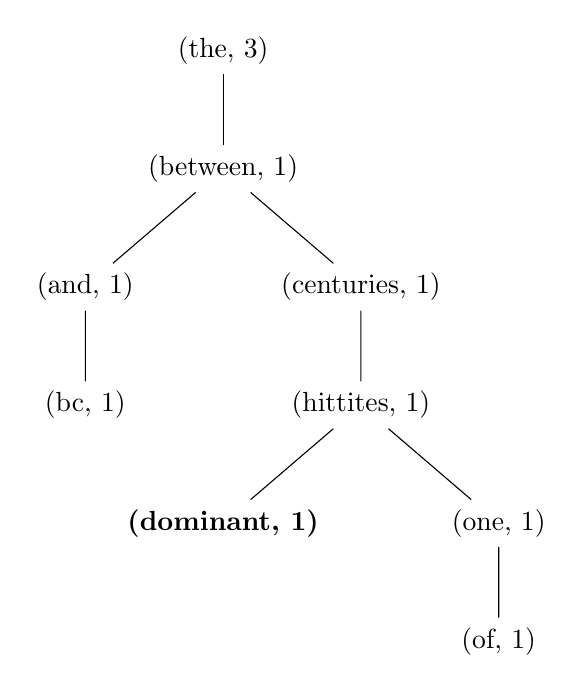
\begin{tikzpicture}
[
    level 1/.style={sibling distance=75mm},
    level 2/.style={sibling distance=35mm},
]
\node { (the, 3)} 
    child {node{ (between, 1)} 
    child {node{ (and, 1)} 
    child {node{ (bc, 1)} 
}}    child {node{ (centuries, 1)} 
    child {node{ (hittites, 1)} 
    child {node{\bfseries (dominant, 1)} 
}    child {node{ (one, 1)} 
    child {node{ (of, 1)} 
}}}}};
\end{tikzpicture}
}
\end{center}

\end{tcolorbox}\subsection{« powers »}
\begin{tcolorbox}[arc=5pt, colback=white!0, colframe=orange!50!black]
\infbox{
Insertion de \textbf{« powers »}
}
\begin{center}
\tbox{
\begin{tikzpicture}
[
    level 1/.style={sibling distance=75mm},
    level 2/.style={sibling distance=35mm},
]
\node { (the, 3)} 
    child {node{ (between, 1)} 
    child {node{ (and, 1)} 
    child {node{ (bc, 1)} 
}}    child {node{ (centuries, 1)} 
    child {node{ (hittites, 1)} 
    child {node{ (dominant, 1)} 
}    child {node{ (one, 1)} 
    child {node{ (of, 1)} 
}    child {node{\bfseries (powers, 1)} 
}}}}};
\end{tikzpicture}
}
\end{center}

\end{tcolorbox}\subsection{« of »}
\begin{tcolorbox}[arc=5pt, colback=white!0, colframe=orange!50!black]
\infbox{
Insertion de \textbf{« of »}
}
\begin{center}
\tbox{
\begin{tikzpicture}
[
    level 1/.style={sibling distance=75mm},
    level 2/.style={sibling distance=35mm},
]
\node { (the, 3)} 
    child {node{ (between, 1)} 
    child {node{ (and, 1)} 
    child {node{ (bc, 1)} 
}}    child {node{ (centuries, 1)} 
    child {node{ (hittites, 1)} 
    child {node{ (dominant, 1)} 
}    child {node{ (one, 1)} 
    child {node{\bfseries (of, 2)} 
}    child {node{ (powers, 1)} 
}}}}};
\end{tikzpicture}
}
\end{center}

\end{tcolorbox}
\subsection{« the »}
\begin{tcolorbox}[arc=5pt, colback=white!0, colframe=orange!50!black]
\infbox{
Insertion de \textbf{« the »}
}
\begin{center}
\tbox{
\begin{tikzpicture}
[
    level 1/.style={sibling distance=75mm},
    level 2/.style={sibling distance=35mm},
]
\node {\bfseries (the, 4)} 
    child {node{ (between, 1)} 
    child {node{ (and, 1)} 
    child {node{ (bc, 1)} 
}}    child {node{ (centuries, 1)} 
    child {node{ (hittites, 1)} 
    child {node{ (dominant, 1)} 
}    child {node{ (one, 1)} 
    child {node{ (of, 2)} 
}    child {node{ (powers, 1)} 
}}}}};
\end{tikzpicture}
}
\end{center}

\end{tcolorbox}
\subsection{« near »}
\begin{tcolorbox}[arc=5pt, colback=white!0, colframe=orange!50!black]
\infbox{
Insertion de \textbf{« near »}
}
\begin{center}
\tbox{
\begin{tikzpicture}
[
    level 1/.style={sibling distance=75mm},
    level 2/.style={sibling distance=35mm},
]
\node { (the, 4)} 
    child {node{ (between, 1)} 
    child {node{ (and, 1)} 
    child {node{ (bc, 1)} 
}}    child {node{ (centuries, 1)} 
    child {node{ (hittites, 1)} 
    child {node{ (dominant, 1)} 
}    child {node{ (one, 1)} 
    child {node{ (of, 2)} 
    child {node{\bfseries (near, 1)} 
}}    child {node{ (powers, 1)} 
}}}}};
\end{tikzpicture}
}
\end{center}

\end{tcolorbox}\subsection{« east »}
\begin{tcolorbox}[arc=5pt, colback=white!0, colframe=orange!50!black]
\infbox{
Insertion de \textbf{« east »}
}
\begin{center}
\tbox{
\begin{tikzpicture}
[
    level 1/.style={sibling distance=75mm},
    level 2/.style={sibling distance=35mm},
]
\node { (the, 4)} 
    child {node{ (between, 1)} 
    child {node{ (and, 1)} 
    child {node{ (bc, 1)} 
}}    child {node{ (centuries, 1)} 
    child {node{ (hittites, 1)} 
    child {node{ (dominant, 1)} 
    child {node{\bfseries (east, 1)} 
}}    child {node{ (one, 1)} 
    child {node{ (of, 2)} 
    child {node{ (near, 1)} 
}}    child {node{ (powers, 1)} 
}}}}};
\end{tikzpicture}
}
\end{center}

\end{tcolorbox}\subsection{« coming »}
\begin{tcolorbox}[arc=5pt, colback=white!0, colframe=orange!50!black]
\infbox{
Insertion de \textbf{« coming »}
}
\begin{center}
\tbox{
\begin{tikzpicture}
[
    level 1/.style={sibling distance=75mm},
    level 2/.style={sibling distance=35mm},
]
\node { (the, 4)} 
    child {node{ (between, 1)} 
    child {node{ (and, 1)} 
    child {node{ (bc, 1)} 
}}    child {node{ (centuries, 1)} 
    child {node{ (hittites, 1)} 
    child {node{ (dominant, 1)} 
    child {node{\bfseries (coming, 1)} 
}    child {node{ (east, 1)} 
}}    child {node{ (one, 1)} 
    child {node{ (of, 2)} 
    child {node{ (near, 1)} 
}}    child {node{ (powers, 1)} 
}}}}};
\end{tikzpicture}
}
\end{center}

\end{tcolorbox}\subsection{« into »}
\begin{tcolorbox}[arc=5pt, colback=white!0, colframe=orange!50!black]
\infbox{
Insertion de \textbf{« into »}
}
\begin{center}
\tbox{
\begin{tikzpicture}
[
    level 1/.style={sibling distance=75mm},
    level 2/.style={sibling distance=35mm},
]
\node { (the, 4)} 
    child {node{ (between, 1)} 
    child {node{ (and, 1)} 
    child {node{ (bc, 1)} 
}}    child {node{ (centuries, 1)} 
    child {node{ (hittites, 1)} 
    child {node{ (dominant, 1)} 
    child {node{ (coming, 1)} 
}    child {node{ (east, 1)} 
}}    child {node{ (one, 1)} 
    child {node{ (of, 2)} 
    child {node{ (near, 1)} 
    child {node{\bfseries (into, 1)} 
}}}    child {node{ (powers, 1)} 
}}}}};
\end{tikzpicture}
}
\end{center}

\end{tcolorbox}\subsection{« conflict »}
\begin{tcolorbox}[arc=5pt, colback=white!0, colframe=orange!50!black]
\infbox{
Insertion de \textbf{« conflict »}
}
\begin{center}
\tbox{
\begin{tikzpicture}
[
    level 1/.style={sibling distance=75mm},
    level 2/.style={sibling distance=35mm},
]
\node { (the, 4)} 
    child {node{ (between, 1)} 
    child {node{ (and, 1)} 
    child {node{ (bc, 1)} 
}}    child {node{ (centuries, 1)} 
    child {node{ (hittites, 1)} 
    child {node{ (dominant, 1)} 
    child {node{ (coming, 1)} 
    child {node{\bfseries (conflict, 1)} 
}}    child {node{ (east, 1)} 
}}    child {node{ (one, 1)} 
    child {node{ (of, 2)} 
    child {node{ (near, 1)} 
    child {node{ (into, 1)} 
}}}    child {node{ (powers, 1)} 
}}}}};
\end{tikzpicture}
}
\end{center}

\end{tcolorbox}\subsection{« with »}
\begin{tcolorbox}[arc=5pt, colback=white!0, colframe=orange!50!black]
\infbox{
Insertion de \textbf{« with »}
}
\begin{center}
\tbox{
\begin{tikzpicture}
[
    level 1/.style={sibling distance=75mm},
    level 2/.style={sibling distance=35mm},
]
\node { (the, 4)} 
    child {node{ (between, 1)} 
    child {node{ (and, 1)} 
    child {node{ (bc, 1)} 
}}    child {node{ (centuries, 1)} 
    child {node{ (hittites, 1)} 
    child {node{ (dominant, 1)} 
    child {node{ (coming, 1)} 
    child {node{ (conflict, 1)} 
}}    child {node{ (east, 1)} 
}}    child {node{ (one, 1)} 
    child {node{ (of, 2)} 
    child {node{ (near, 1)} 
    child